\begin{figure}
    \centering
    {\small
    \begin{subfigure}{.5\textwidth}
    \begin{centering}
    % 
    $ 
    \begin{array}{l}
      \kw{nestedW}(k) \triangleq \\
      \clabel{\assign{i}{k} }^{0} ; 
      \clabel{ \assign{x}{\query(\chi[0])}}^{1} ; 
      \clabel{ \assign{y}{\query(\chi[1])}}^{2} ; \\
          \ewhile ~ \clabel{i > 0}^{3} ~ \edo ~ \\
          \Big(
           \clabel{\assign{i}{i-1}}^{4} ;
           \clabel{\assign{j}{k}}^{5} ;
           \clabel{\assign{y}{\query(\chi(\ln(x) + y))} }^{6}  ; \\
           \ewhile ~ \clabel{j > 0}^{7} ~ \edo ~ \\
           \Big(
            \clabel{\assign{j}{j-1}}^{8};
            \clabel{\assign{x}{\query(\chi(\ln(y))+\chi[x])} }^{9}
            \Big) \Big)
      \end{array}
    %       
    $
    \caption{}
    \end{centering}
    \end{subfigure}
    \quad
    \begin{subfigure}{.3\textwidth}
      \begin{centering}
      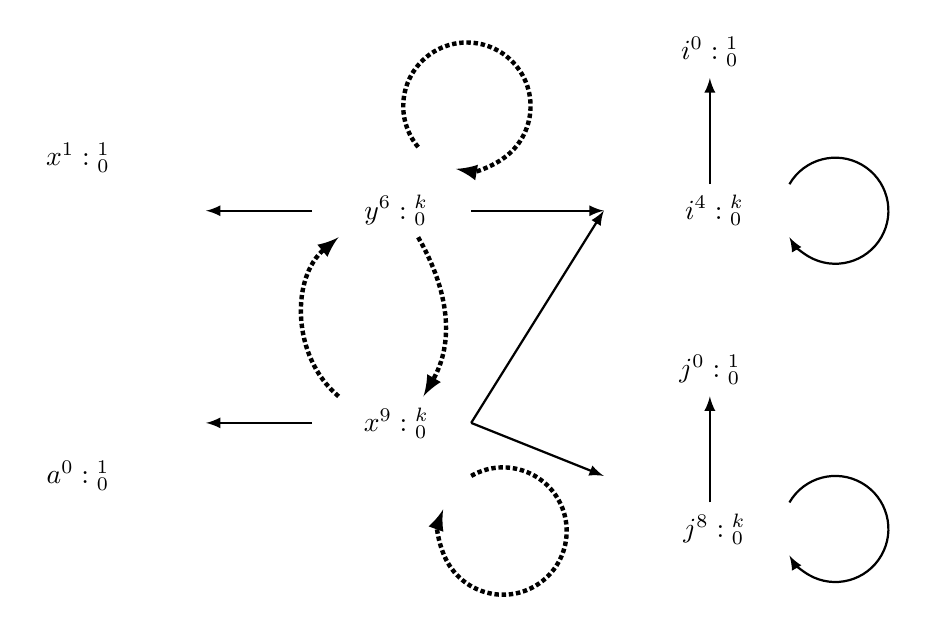
\begin{tikzpicture}[scale=\textwidth/18cm,samples=200]
% Variables Initialization
\draw[] (-6, 1) circle (0pt) node{{ $a^0: {}^1_{0}$}};
\draw[] (-6, 7) circle (0pt) node{{ $x^1: {}^{1}_{0}$}};
% Variables Inside the Loop
   \draw[] (0, 6) circle (0pt) node{{ $y^6: {}^{k}_{0}$}};
   \draw[] (0, 2) circle (0pt) node{{ $x^9: {}^{k}_{0}$}};
   % Counter Variables
   \draw[] (6, 9) circle (0pt) node {{$i^0: {}^{1}_{0}$}};
   \draw[] (6, 6) circle (0pt) node {{ $i^4: {}^{k}_{0}$}};
   \draw[] (6, 3) circle (0pt) node {{$j^0: {}^{1}_{0}$}};
   \draw[] (6, 0) circle (0pt) node {{ $j^8: {}^{k}_{0}$}};
   %
   % Value Dependency Edges:
   \draw[ ultra thick, -latex, densely dotted,] (0.5, 7.2) arc (220:-100:1.2);
   \draw[ thick, -latex] (6, 6.5)  -- (6, 8.5) ;
   \draw[ thick, -latex] (6, 0.5)  -- (6, 2.5) ;
   \draw[ ultra thick, -latex, densely dotted,] (1.5, 1.0) arc (120:-200:1.2);
   % Value Dependency Edges on Initial Values:
   \draw[ thick, -latex,] (-1.5, 2)  -- (-3.5, 2) ;
   \draw[ thick, -latex,] (-1.5, 6)  -- (-3.5, 6) ;
   %
   \draw[ ultra thick, -latex, densely dotted,] (-1, 2.5)  to  [out=-220,in=220]  (-1, 5.5);
   \draw[ ultra thick, -latex, densely dotted,]  (0.5, 5.5) to  [out=-60,in=60] (0.6, 2.5) ;
   % Control Dependency
  %  \draw[ thick,-latex] (1.5, 7)  -- (4, 9) ;
  %  \draw[ thick,-latex] (1.5, 4)  -- (4, 9) ;
  \draw[ thick, -latex, ] (7.5, 6.5) arc (150:-150:1);
  \draw[ thick, -latex, ] (7.5, 0.5) arc (150:-150:1);
  \draw[ thick,-latex] (1.5, 6)  -- (4, 6) ;
   \draw[ thick,-latex] (1.5, 2)  -- (4, 6) ;
   \draw[ thick,-latex] (1.5, 2)  -- (4, 1) ;
   \end{tikzpicture}
   \caption{}
      \end{centering}
      \end{subfigure}
    }
    \vspace{-0.4cm}
     \caption{(a) The nested while loop example, (b) The estimated dependency graph generated from $\THESYSTEM$.}
    \label{fig:alg_adaptsearch_nestedwhile}
    \end{figure}